
\section{Editor and REPL console}

Creation of a user-friendly interface was an important part of the project.
The greatest challenge lied in finding the most intuitive way of presenting a complicated and highly advanced system. The main component was the language of regular expressions itself. The user should be able to edit its code with ease. The second key feature was the ability to execute the code. 
In many Turing-complete languages, every expression can be evaluated into some value, which could then be printed back to the user. For example in python's REPL, typing $2+2$ yields $4$.
\begin{lstlisting}
	>>> 2 + 2
	4
\end{lstlisting}
In a more complicated case like running a regex, user obtains an object containing all matched groups
\begin{lstlisting}
	>>> re.compile('a|b*').match('xxaxxbxxbbbx')
	<re.Match object; span=(0, 0), match=''>
\end{lstlisting}
In Solomonoff the problem is not so trivial. The regular expressions could in principle be evaluated down to formal languages. For example 
\begin{lstlisting}
	'a' ('b' | 'c' | 'ef' ) 'd'
\end{lstlisting}
would return a language consisting of strings
\begin{lstlisting}
	'abd', 'acd', 'aefd'
\end{lstlisting}
The issue wish such approach is that not all languages are finite. The expression
\begin{lstlisting}
	'a'*
\end{lstlisting}
would be evaluated as infinite set
\begin{lstlisting}
	'', 'a', 'aa', 'aaa', ...
\end{lstlisting}
Some regexes, might be finite but of exponential size. For instance
\begin{lstlisting}
	('0' | '1') ('0' | '1') ('0' | '1') ('0' | '1')
\end{lstlisting}
yields a set of all bit-strings of length 4. Presenting the user with the result in the form of formal languages would be often impractical or impossible. 

As a result, our REPL does not evaluate expressions. The results of compilation are not printed in any form. Instead the interface is meant to be silent when compilation is successful. Only errors are printed. 

There are many different approaches to implement the user interface for REPL.
One of them would be having a single editor window with all the code in it and the REPL output printed on the margins next to each respective line. This provides a very immersive user experience for Turing-complete languages. Such an approach has been chosen by many debuggers, including the one presented in figure \ref{intellij_debug}.
\begin{figure}[h]
	\centering
	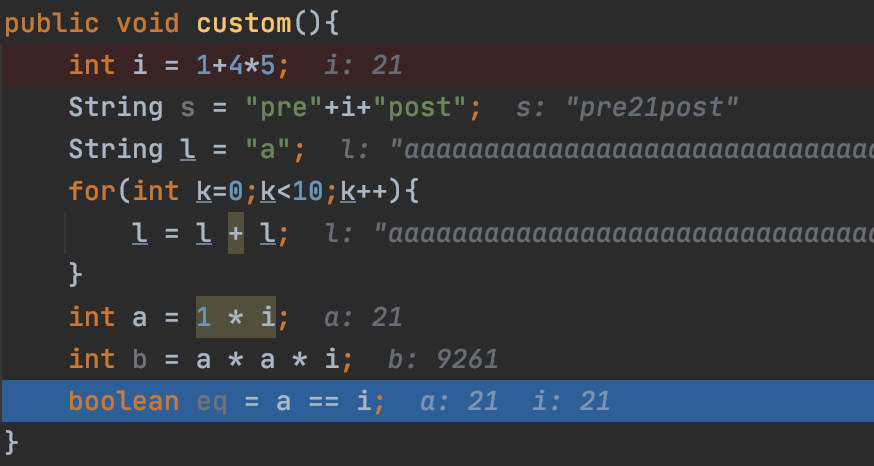
\includegraphics[scale=0.85]{java_repl.png}
	\caption{Graphical interface of debugger used by IntelliJ. The results of Java expressions are displayed in the same line. The contents can change dynamically as the execution progresses.}
	\label{intellij_debug}
\end{figure}
For regular expressions such an approach is not as spectacular. 
It's not possible to evaluate a regex down into any particular value.
The closest two operations that could be used for presentation purposes are as follows. Its either possible to evaluate a regular expression on a particular input (it can be achieved with \texttt{:eval NAME 'input string'} command in REPL) or generate a sample set of accepted inputs (using \texttt{:rand\_sample NAME of\_size NUMBER} ).

One last and perhaps the most engaging way of presenting the results to the user is by visually graphing them.
Any automata can be interpreted as a directed graph. This property  was used to further enhance user interface (automaton graph will be shown after typing \texttt{:vis NAME} or by clicking an appropriate button in the graphical interface)

Those and many other functionalities have been added to the browser-based version of REPL. Its implementation is not trivial. One of the ways to achieve such results would be by implementing a parser that could halt mid-parsing. For example user could first type
\begin{lstlisting}
	x = ('x' |
\end{lstlisting}
and hit the return button. The parser should notice that the expression is not finished and it has to wait for the next line of input.  Then as the user types the next line
\begin{lstlisting}
	'y' )
\end{lstlisting}
a full and valid expression could be recognised and parser could return.
This approach is used by some programming languages. It's difficult to implement and requires the grammar to be appropriately structured. We later abandoned this idea due to the problematic nature of Solomonoff's grammar. In particular, it does not use semicolons to separate statements. For example
\begin{lstlisting}
	x = 'a' 
	y = 'b'
\end{lstlisting}
could be written in a single line
\begin{lstlisting}
	x = 'a' y = 'b'
\end{lstlisting}
The equality sign determines the start of a new statement. By its very nature, parsing such grammars, requires a lookahead of one token into the future. When the input is read in fragments, line by line, such a lookahead is not possible to obtain.
User could first type
\begin{lstlisting}
	x = 'a' y
\end{lstlisting}
which would be recognized by the parser as concatenation of string    \texttt{'a'} with variable  \texttt{y}. If the user then types
\begin{lstlisting}
	= 'b'
\end{lstlisting}
in the upcoming line, then the previous results of parsing would have to be discarded and the entire input reparsed again. Hence we decided to simplify the REPL and assume that every line of input fully defines the entirety of expression. As a result it's not possible to split input into multiple lines when using console. This is not a serious limitation, because multiline expressions could still be written in the editor window instead of console. 

The division of user interface into editor and console has one more advantage. It closely mimics the layout of the command-line interface, where the typical workflow is to edit source code in local files using any text editor of user's choice and the REPL is kept open all the time alongside the editor. Many existing modes for Emacs follow a similar convention.

\section{Spring backend}

A Spring MVC is a Java framework which is used to build web applications. It follows the Model-View-Controller design pattern. It implements all the basic features of a core spring framework like Inversion of Control, Dependency Injection.
A Spring MVC provides an elegant solution to use MVC in spring framework by the help of DispatcherServlet. Here, DispatcherServlet is a class that receives the incoming request and maps it to the right resource such as controllers, models, and views.



\tikzset{every picture/.style={line width=0.75pt}} %set default line width to 0.75pt        

\begin{tikzpicture}[x=0.75pt,y=0.75pt,yscale=-1,xscale=1]
	%uncomment if require: \path (0,235); %set diagram left start at 0, and has height of 235
	
	
	% Text Node
	\draw (300,57) node    {$Web\ browser$};
	% Text Node
	\draw (109,176) node    {$Frontend\ controller$};
	% Text Node
	\draw (516,173) node    {$View$};
	% Text Node
	\draw (320,176) node    {$Controller$};
	% Text Node
	\draw (721,21) node    {$0$};
	% Text Node
	\draw (701,71) node    {$0$};
	% Connection
	\draw    (324.11,69.95) -- (494,161.19) ;
	\draw [shift={(322.34,69)}, rotate = 28.24] [color={rgb, 255:red, 0; green, 0; blue, 0 }  ][line width=0.75]    (10.93,-3.29) .. controls (6.95,-1.4) and (3.31,-0.3) .. (0,0) .. controls (3.31,0.3) and (6.95,1.4) .. (10.93,3.29)   ;
	% Connection
	\draw    (280.74,69) -- (129.96,162.94) ;
	\draw [shift={(128.26,164)}, rotate = 328.08000000000004] [color={rgb, 255:red, 0; green, 0; blue, 0 }  ][line width=0.75]    (10.93,-3.29) .. controls (6.95,-1.4) and (3.31,-0.3) .. (0,0) .. controls (3.31,0.3) and (6.95,1.4) .. (10.93,3.29)   ;
	% Connection
	\draw    (180,176) -- (278.5,176) ;
	\draw [shift={(280.5,176)}, rotate = 180] [color={rgb, 255:red, 0; green, 0; blue, 0 }  ][line width=0.75]    (10.93,-3.29) .. controls (6.95,-1.4) and (3.31,-0.3) .. (0,0) .. controls (3.31,0.3) and (6.95,1.4) .. (10.93,3.29)   ;
	% Connection
	\draw    (492,173.37) -- (359.5,175.4) ;
	\draw [shift={(494,173.34)}, rotate = 179.12] [color={rgb, 255:red, 0; green, 0; blue, 0 }  ][line width=0.75]    (10.93,-3.29) .. controls (6.95,-1.4) and (3.31,-0.3) .. (0,0) .. controls (3.31,0.3) and (6.95,1.4) .. (10.93,3.29)   ;
	
\end{tikzpicture}
Model contains the data of the application. A data can be a single object or a collection of objects. \\
Controller contains the business logic of an application. Here, the @Controller annotation is used to mark the class as the controller. \\
View represents the provided information in a particular format. Generally, JSP+JSTL is used to create a view page. Although Spring also supports other view technologies such as Apache Velocity, Thymeleaf and FreeMarker. \\
Frontend controller is implemented in Spring Web MVC in the form of the DispatcherServlet class. It is responsible to manage the flow of the Spring MVC application.
The flow of Spring Web MVC could be presented as follows
\tikzset{every picture/.style={line width=0.75pt}} %set default line width to 0.75pt        

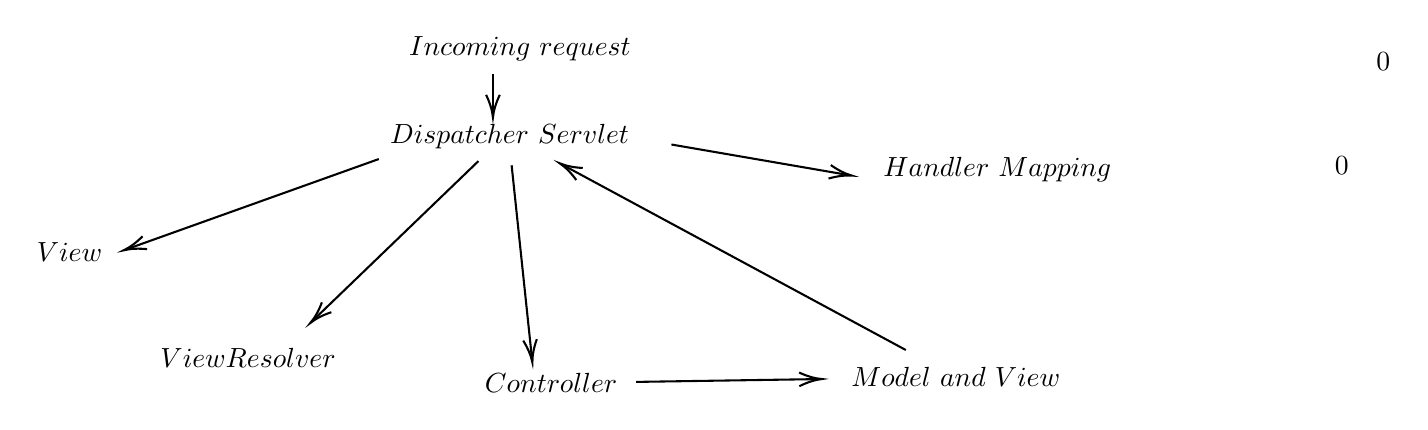
\begin{tikzpicture}[x=0.75pt,y=0.75pt,yscale=-1,xscale=1]
	%uncomment if require: \path (0,235); %set diagram left start at 0, and has height of 235
	
	%Straight Lines [id:da43796635224753366] 
	\draw    (301,71) -- (310.79,164.01) ;
	\draw [shift={(311,166)}, rotate = 263.99] [color={rgb, 255:red, 0; green, 0; blue, 0 }  ][line width=0.75]    (10.93,-3.29) .. controls (6.95,-1.4) and (3.31,-0.3) .. (0,0) .. controls (3.31,0.3) and (6.95,1.4) .. (10.93,3.29)   ;
	%Straight Lines [id:da8543300973373011] 
	\draw    (285,69) -- (205.44,145.61) ;
	\draw [shift={(204,147)}, rotate = 316.08000000000004] [color={rgb, 255:red, 0; green, 0; blue, 0 }  ][line width=0.75]    (10.93,-3.29) .. controls (6.95,-1.4) and (3.31,-0.3) .. (0,0) .. controls (3.31,0.3) and (6.95,1.4) .. (10.93,3.29)   ;
	%Straight Lines [id:da26721417437109896] 
	\draw    (237,68) -- (115.88,111.33) ;
	\draw [shift={(114,112)}, rotate = 340.32] [color={rgb, 255:red, 0; green, 0; blue, 0 }  ][line width=0.75]    (10.93,-3.29) .. controls (6.95,-1.4) and (3.31,-0.3) .. (0,0) .. controls (3.31,0.3) and (6.95,1.4) .. (10.93,3.29)   ;
	%Straight Lines [id:da24273477514405806] 
	\draw    (378,61) -- (463.03,75.66) ;
	\draw [shift={(465,76)}, rotate = 189.78] [color={rgb, 255:red, 0; green, 0; blue, 0 }  ][line width=0.75]    (10.93,-3.29) .. controls (6.95,-1.4) and (3.31,-0.3) .. (0,0) .. controls (3.31,0.3) and (6.95,1.4) .. (10.93,3.29)   ;
	%Straight Lines [id:da4809109559432261] 
	\draw    (292,27) -- (292,46) ;
	\draw [shift={(292,48)}, rotate = 270] [color={rgb, 255:red, 0; green, 0; blue, 0 }  ][line width=0.75]    (10.93,-3.29) .. controls (6.95,-1.4) and (3.31,-0.3) .. (0,0) .. controls (3.31,0.3) and (6.95,1.4) .. (10.93,3.29)   ;
	
	% Text Node
	\draw (300,57) node    {$\text{Dispatcher\ Servlet}$};
	% Text Node
	\draw (515,173) node    {$\text{Model\ and\ View}$};
	% Text Node
	\draw (320,176) node    {$\text{Controller}$};
	% Text Node
	\draw (721,21) node    {$0$};
	% Text Node
	\draw (701,71) node    {$0$};
	% Text Node
	\draw (174,164) node    {$\text{ViewResolver}$};
	% Text Node
	\draw (88,113) node    {$\text{View}$};
	% Text Node
	\draw (535,73) node    {$\text{Handler\ Mapping}$};
	% Text Node
	\draw (305,15) node    {$\text{Incoming\ request}$};
	% Connection
	\draw    (325.85,70.95) -- (490.91,160) ;
	\draw [shift={(324.09,70)}, rotate = 28.35] [color={rgb, 255:red, 0; green, 0; blue, 0 }  ][line width=0.75]    (10.93,-3.29) .. controls (6.95,-1.4) and (3.31,-0.3) .. (0,0) .. controls (3.31,0.3) and (6.95,1.4) .. (10.93,3.29)   ;
	% Connection
	\draw    (448.5,174.02) -- (361,175.37) ;
	\draw [shift={(450.5,173.99)}, rotate = 179.12] [color={rgb, 255:red, 0; green, 0; blue, 0 }  ][line width=0.75]    (10.93,-3.29) .. controls (6.95,-1.4) and (3.31,-0.3) .. (0,0) .. controls (3.31,0.3) and (6.95,1.4) .. (10.93,3.29)   ;
	
\end{tikzpicture}
As displayed in the figure, all the incoming requests are intercepted by the DispatcherServlet that works as the front controller.
The DispatcherServlet gets an entry of handler mapping from the XML file and forwards the request to the controller.
The controller returns an object of ModelAndView.
The DispatcherServlet checks the entry of the view resolver in the XML file and invokes the specified view component.

Using Spring MVC comes with numerous advantages. It allows for separation of roles, where the model object, controller, command object, view resolver, DispatcherServlet, validator, etc. can be fulfilled by a specialized object. It uses a light-weight servlet container to develop and deploy your application.
It provides a robust configuration for both framework and application classes that includes easy referencing across contexts, such as from web controllers to business objects and validators.
The Spring MVC also facilitates fast and parallel development.
It promotes reusable business code by using the existing business objects instead of creating new ones.
Test of JavaBean classes enables injection of test data using the setter methods, which allows for easier testing.
Flexible Mappings provide the specific annotations that easily redirect the page.
Overall Spring is a powerful tool used by numerous companies and developers around the world.



In this project, Spring has been used to facilitate communication between frontend interface and compiler instances. The REPL is implemented on the server-side as a REST API endpoint. 
\begin{lstlisting}
	@PostMapping("/repl")
	public ReplResponse repl(HttpSession httpSession, 
	@RequestBody String line)
\end{lstlisting}
Every user has their own instance of REPL
\begin{lstlisting}
	Repl repl = (Repl) httpSession.getAttribute("repl");
\end{lstlisting}
which holds a reference to the compiler and a set of built-in commands
\begin{lstlisting}
	public static class Repl {
		private static class CmdMeta<Result> {
			final ReplCommand<Result> cmd;
			final String help;
			final String template;
			
			private CmdMeta(ReplCommand<Result> cmd, 
			String help, String template) {
				this.cmd = cmd;
				this.help = help;
				this.template = template;
			}
		}
		
		HashMap<String, Repl.CmdMeta<String>> commands;
		OptimisedHashLexTransducer compiler;
	}
\end{lstlisting}
whenever user types some command on the REPL console
\begin{lstlisting}
	:cmd arg1 arg2 arg3
\end{lstlisting}
it gets parsed as
\begin{lstlisting}
	String firstWord = "cmd";
	String remaining = "arg1 arg2 arg3";
\end{lstlisting}
and then the appropriate command implementation is looked up in the map
\begin{lstlisting}
	final Repl.CmdMeta<String> cmd = commands.get(firstWord);
	return cmd.cmd.run(httpSession, compiler, log, debug, remaining);
\end{lstlisting}
The rest controller contains implementations of many such commands
\begin{lstlisting}
	public static final ReplCommand<String> REPL_LIST = ...
	public static final ReplCommand<String> REPL_EVAL = ...
	public static final ReplCommand<String> REPL_RUN = ...
	public static final ReplCommand<String> REPL_EXPORT = ..
	public static final ReplCommand<String> REPL_IS_DETERMINISTIC = ...
	public static final ReplCommand<String> REPL_LIST_PIPES = ...
	public static final ReplCommand<String> REPL_EQUAL = ...
	public static final ReplCommand<String> REPL_RAND_SAMPLE = ...
	public static final ReplCommand<String> REPL_CLEAR = ...
	public static final ReplCommand<String> REPL_UNSET = ...
	public static final ReplCommand<String> REPL_RESET = ...
	public static final ReplCommand<String> REPL_LOAD = ...
	public static final ReplCommand<String> REPL_VIS = ...
\end{lstlisting}
All of those definitions above are lambda expressions that use library functions
of the compiler. The parameters taken by those lambda expressions are as follows
\begin{lstlisting}
	public interface ReplCommand<Result> {
		Result run(
		HttpSession httpSession, 
		OptimisedHashLexTransducer compiler, 
		Consumer<String> log, 
		Consumer<String> debug, 
		String args) throws Exception;
	}
\end{lstlisting}
As an example, consider the command 
\begin{lstlisting}
	:eval f 'abc'
\end{lstlisting}
which evaluates transducer   \texttt{f} for input string    \texttt{'abc'}. 
On the frontend side, JavaScript will perform REST query as follows
\begin{lstlisting}
	const response = await fetch('repl', {
		method: 'POST',
		body: ":eval f 'abc'"
	})
\end{lstlisting}
which will be received by server
\begin{lstlisting}
	@PostMapping("/repl")
	public ReplResponse repl(HttpSession httpSession, 
	@RequestBody String line) {
		Repl repl = (Repl) httpSession.getAttribute("repl");
		final String result = repl.run(
		httpSession, 
		line, // ":eval f 'abc'"
		s -> out.append(s).append('\n'), // console output
		s -> { } // debug logs are not displayed
		);
		...
	}
\end{lstlisting}
and the     \texttt{repl.run} method will query the appropriate implementation to call for
the     \texttt{:eval} command.
\begin{lstlisting}     
	final String firstWord = "eval";
	final String remaining = "f 'abc'";
	final Repl.CmdMeta<String> cmd = commands.get(firstWord);
	return cmd.cmd.run(httpSession, compiler, log, debug, remaining);
\end{lstlisting}
This in turn will trigger the following lambda function
\begin{lstlisting}
	ReplCommand<String> REPL_EVAL = 
	(httpSession, compiler, logs, debug, args) -> {
		String[] parts = args.split("\\s+", 2); // f 'abc'
		String name = parts[0]; // f
		String input = parts[1]; // 'abc'
		G transducer = compiler.getTransducer(name);
		String output = compiler.specs.evaluate(transducer, input);
		return output == null ? "No match!" : output;
	};
\end{lstlisting}
The output is sent back to JavaScript in form of JSON
\begin{lstlisting}
	const replResult = JSON.parse(await response.text())
\end{lstlisting}
Remaining commands are implemented in a similar way.

Several of the functions may require access to HTTP session. In particular it's worth analysing the     \texttt{:load} command. It's purpose is to emulate the process of loading source code from a file. Whenever a user types some code in the editor, it needs to be transported to the server, then parsed and compiled. All the defined transducers results need to be saved for later use. The simplest way of achieving this, would be by extending the REST API as
\begin{lstlisting}
	class ReplInput{
		String command;
		String editorContent;
	}
	public ReplResponse repl(
	HttpSession httpSession, 
	@RequestBody ReplInput)
\end{lstlisting}
and query it using
\begin{lstlisting}
	const response = await fetch('repl', {
		method: 'POST',
		body: {
			command: replCommand,
			editorContent: editor.getValue()
		}
	})
\end{lstlisting}
The downside of such a solution is that the editor content could become large and sending it would require more internet bandwidth and time. Often the user only wants to execute simple short REPL commands that do not require sending the entire code. Sometimes the code might be required but resending it might be omitted as long as the user has not modified it. Hence the process of uploading code to the server has been delegated to a separate REST call.
\begin{lstlisting}
	const response = await fetch('upload_code', {
		method: 'POST',
		body: code
	})
\end{lstlisting}
The code is then stored in HTTP session, so the REST endpoint has a very simple implementation
\begin{lstlisting}
	@PostMapping("/upload_code")
	public void uploadCode(HttpSession httpSession, 
	@RequestBody String text) {
		httpSession.setAttribute("code", text);
	}
\end{lstlisting}


Aside from the editor and REPL there is one more window on the webpage. It is dedicated to tutorials and short documentation.  While it does not enhance the functionality of the website per se, it plays an important role. The Solomonoff compiler is a very niche and specialised tool. There are no similar tools and any user coming to the website is not expected to be familiar with its usage. The primary purpose of the website is not to be a replacement for the user's IDE and terminal. Instead it serves as an all-in-one introductory tutorial, interactive playground and a marketing campaign. We want to make the learning materials easily accessible and abundant. Building a strong community is the back-bone of every open-source project. 

\section{Design}


The frontend technologies used for designing our website are based on Bootstrap  \cite{bootstrap}. It is an HTML, CSS \& JS Library that focuses on simplifying the development of informative web pages (as opposed to web apps). The primary purpose of adding it to a web project is to apply Bootstrap's choices of color, size, font and layout to that project. As such, the primary factor is whether the developers in charge find those choices to their liking. Once added to a project, Bootstrap provides basic style definitions for all HTML elements. The result is a uniform appearance for prose, tables and form elements across web browsers. In addition, developers can take advantage of CSS classes defined in Bootstrap to further customize the appearance of their contents. For example, Bootstrap has provisioned for light- and dark-colored tables, page headings, more prominent pull quotes, and text with a highlight.
Bootstrap also comes with several JavaScript components in the form of jQuery plugins. They provide additional user interface elements such as dialog boxes, tooltips, and carousels. Each Bootstrap component consists of an HTML structure, CSS declarations, and in some cases accompanying JavaScript code. They also extend the functionality of some existing interface elements, including for example an auto-complete function for input fields.
The most prominent components of Bootstrap are its layout components, as they affect an entire web page. The basic layout component is called "Container", as every other element in the page is placed in it. Developers can choose between a fixed-width container and a fluid-width container. While the latter always fills the width of the web page, the former uses one of the four predefined fixed widths, depending on the size of the screen showing the page:
\begin{itemize}
	\item Smaller than 576 pixels
	\item 576–768 pixels
	\item 768–992 pixels
	\item 992–1200 pixels
	\item Larger than 1200 pixels
\end{itemize}
Once a container is in place, other Bootstrap layout components implement a CSS Flexbox layout through defining rows and columns.
A precompiled version of Bootstrap is available in the form of one CSS file and three JavaScript files that can be readily added to any project. The raw form of Bootstrap, however, enables developers to implement further customization and size optimizations. This raw form is modular, meaning that the developer can remove unneeded components, apply a theme and modify the uncompiled Sass files.

In figure \ref{navbar} is presented an example of a navigation bar created with help of Bootstraps \texttt{nav} classes.
\begin{figure}
	\centering
	
	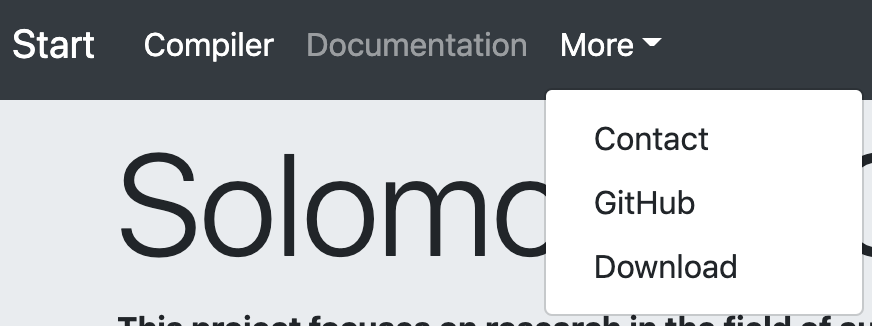
\includegraphics[scale=0.7]{navbar.png}
	\caption{Navigation bar using dedicated Bootstrap classes from the \texttt{nav} family}
	\label{navbar}
\end{figure}
Figure \ref{panes} shows two responsive panes implemented using \texttt{flex}, \texttt{row} and \texttt{column} classes.
\begin{figure}
	\centering
	
	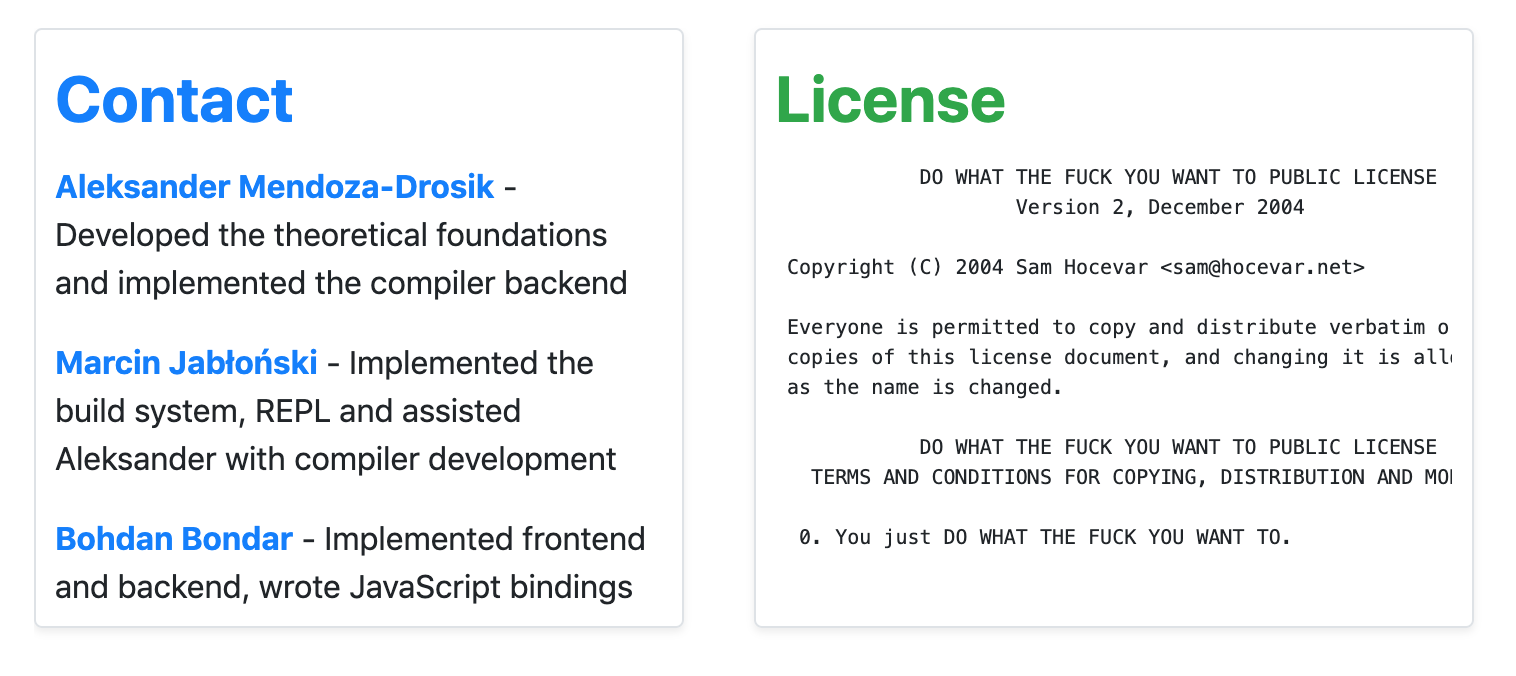
\includegraphics[scale=0.4]{panes.png}
	\caption{The two panes below will change their size and layout depending on dimensions and orientation of the screen.}
	\label{panes}
\end{figure}

Our website has seen numerous design changes. Since the beginning we knew there must be a way to interact with the code but the exact best way of presenting it to the user was not so self-evident. There exist numerous different approaches that are highly dependent on the language. Figure \ref{java_console} shows an example of an online  Java  compiler consisting only of two windows - one for code and one for compiler output.
\begin{figure}
	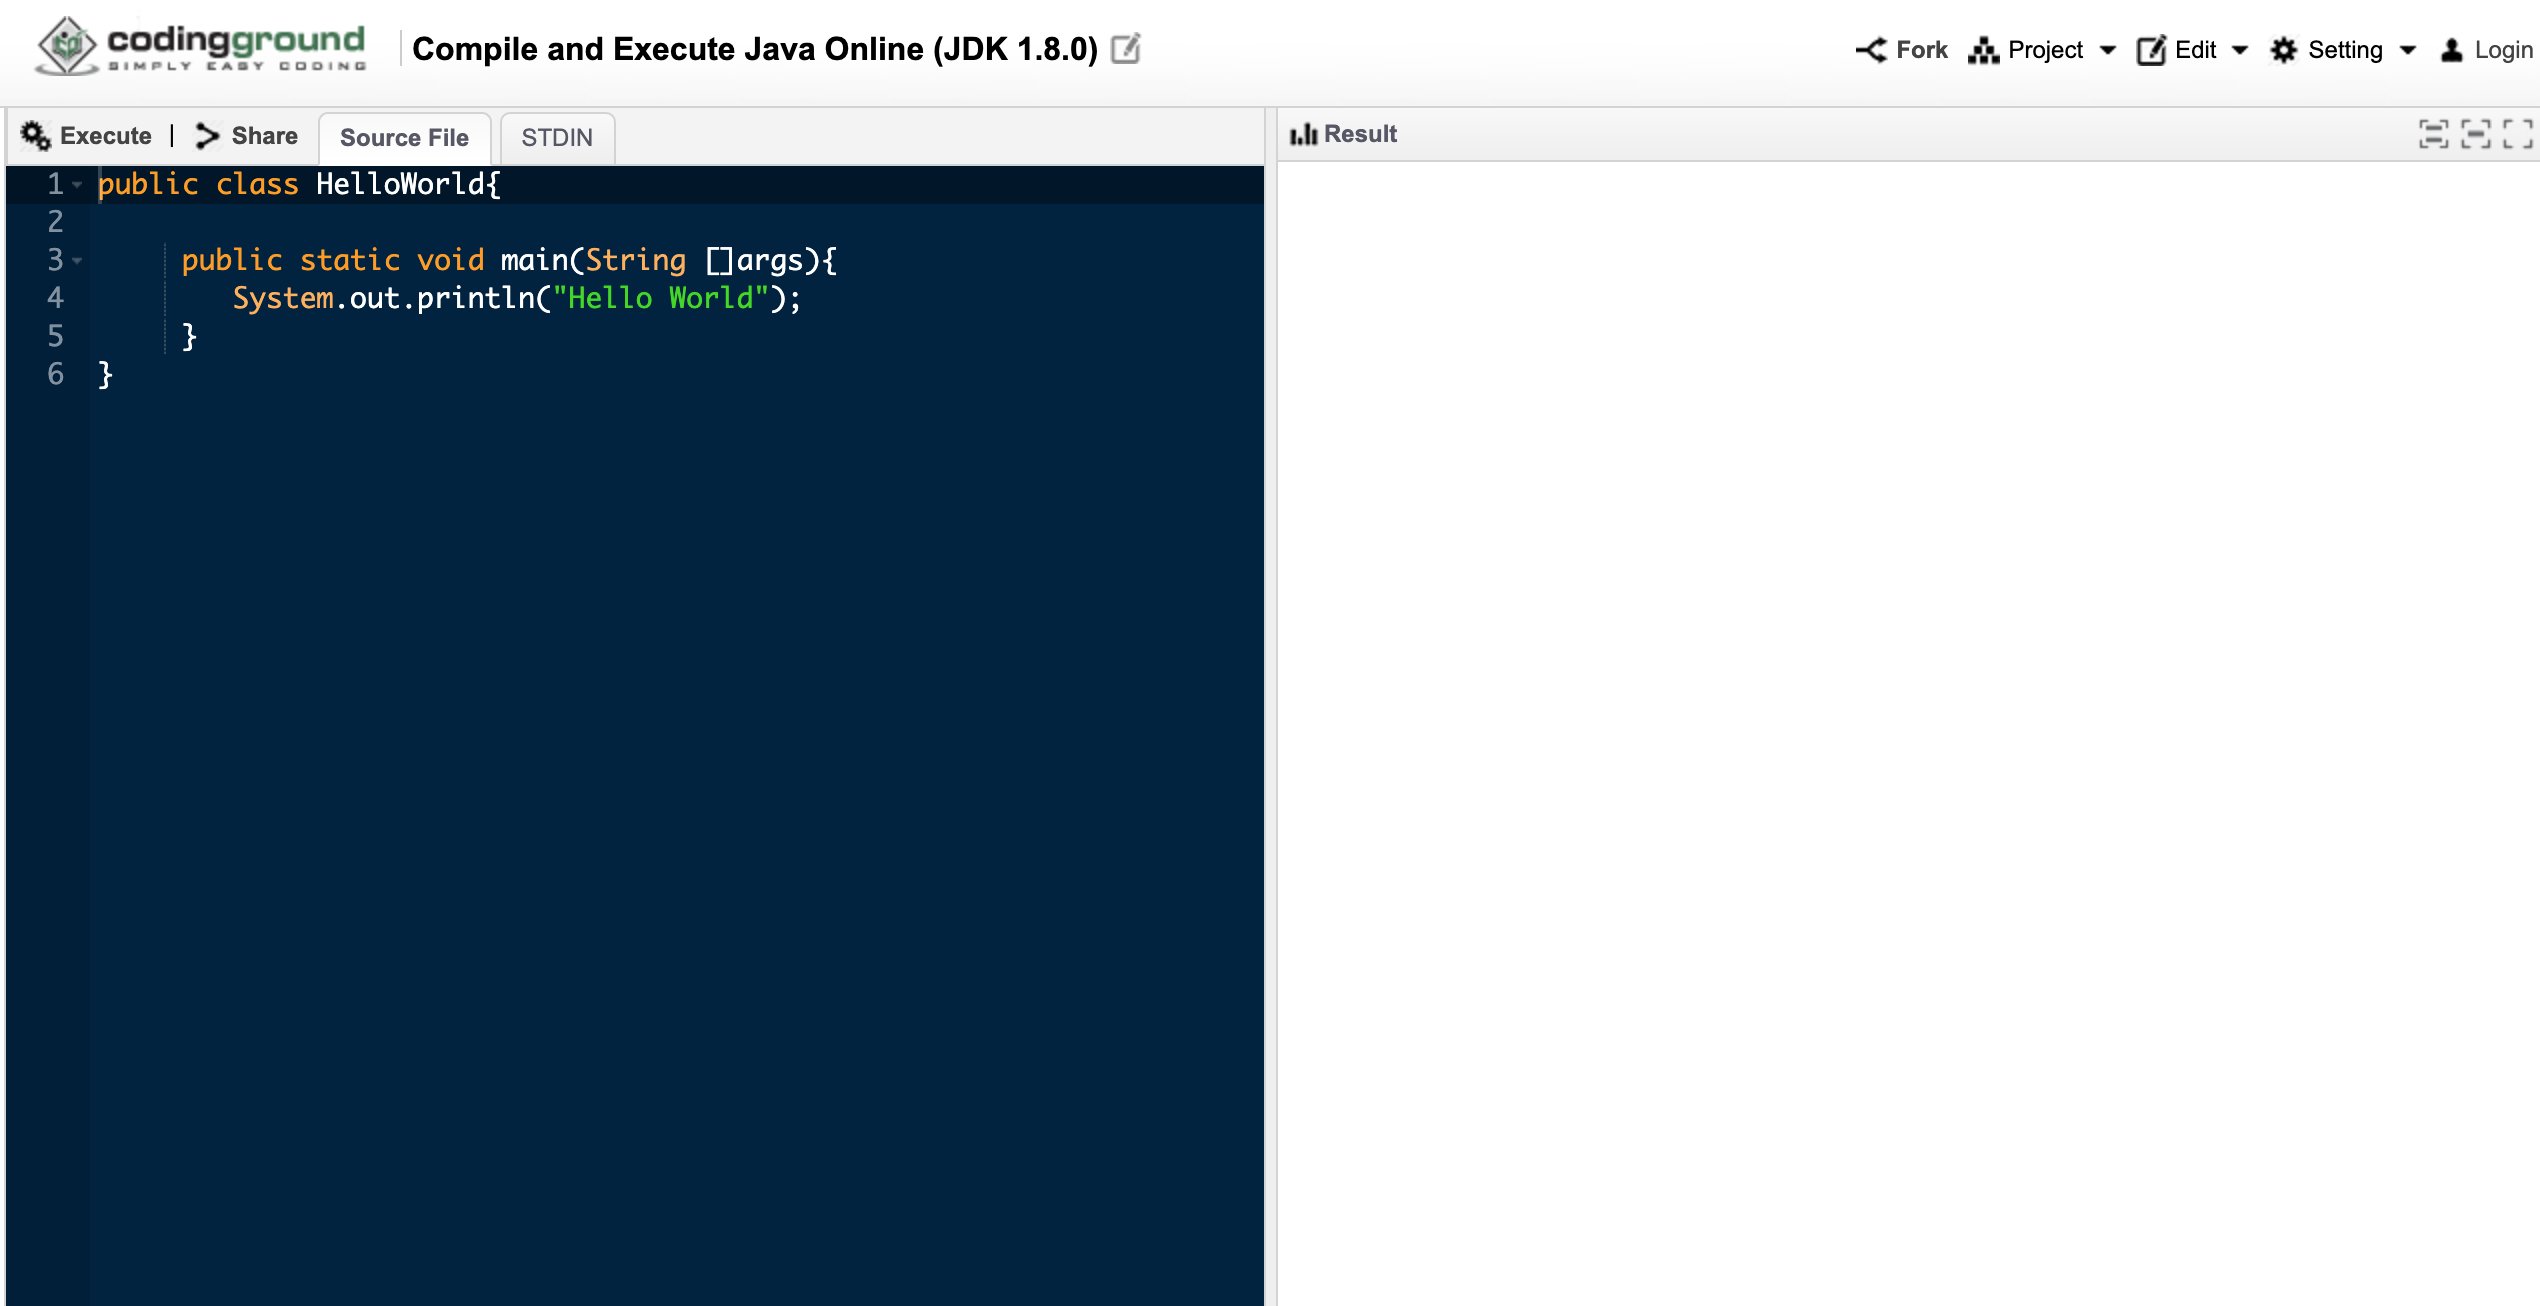
\includegraphics[scale=0.3]{java.png}
	\caption{The CodingGround website provides an online compiler for several languages. This Java example has a dedicated window that emulates terminal output.}
	\label{java_console}
\end{figure}
Java does not have REPL, hence there is no need to implement console input.
A slightly different approach has been taken by Haskell mode for emacs presented in figure \ref{haskell_repl}. 
\begin{figure}
	\centering
	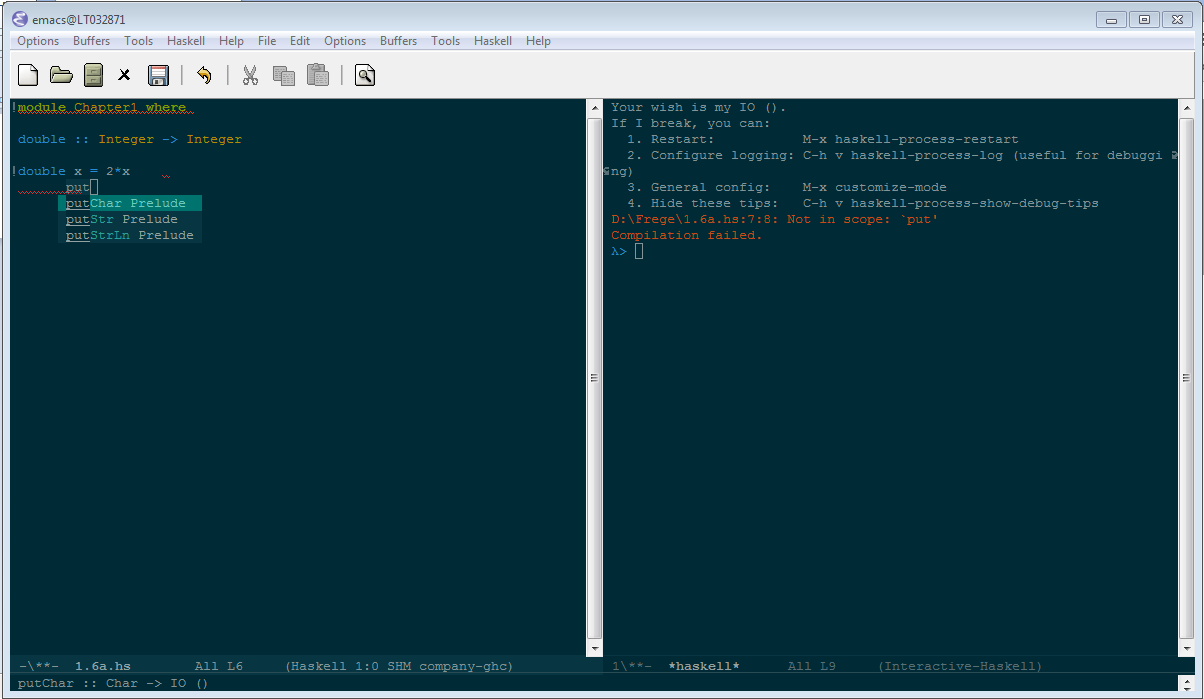
\includegraphics[scale=0.45]{haskell.png}
	\caption{A dedicated Emacs mode for Haskell allows for interactive testing and evaluation of arbitrary expression defined in the source file.}
	\label{haskell_repl}
\end{figure}
There it is indeed possible to evaluate smaller snippets of code in the right window, while the left one is solely dedicated to editing local files that can be saved persistently. Figure \ref{final} presents the approach that we settled for in the final version of the online playground for Solomonoff.
\begin{figure}
	\centering
	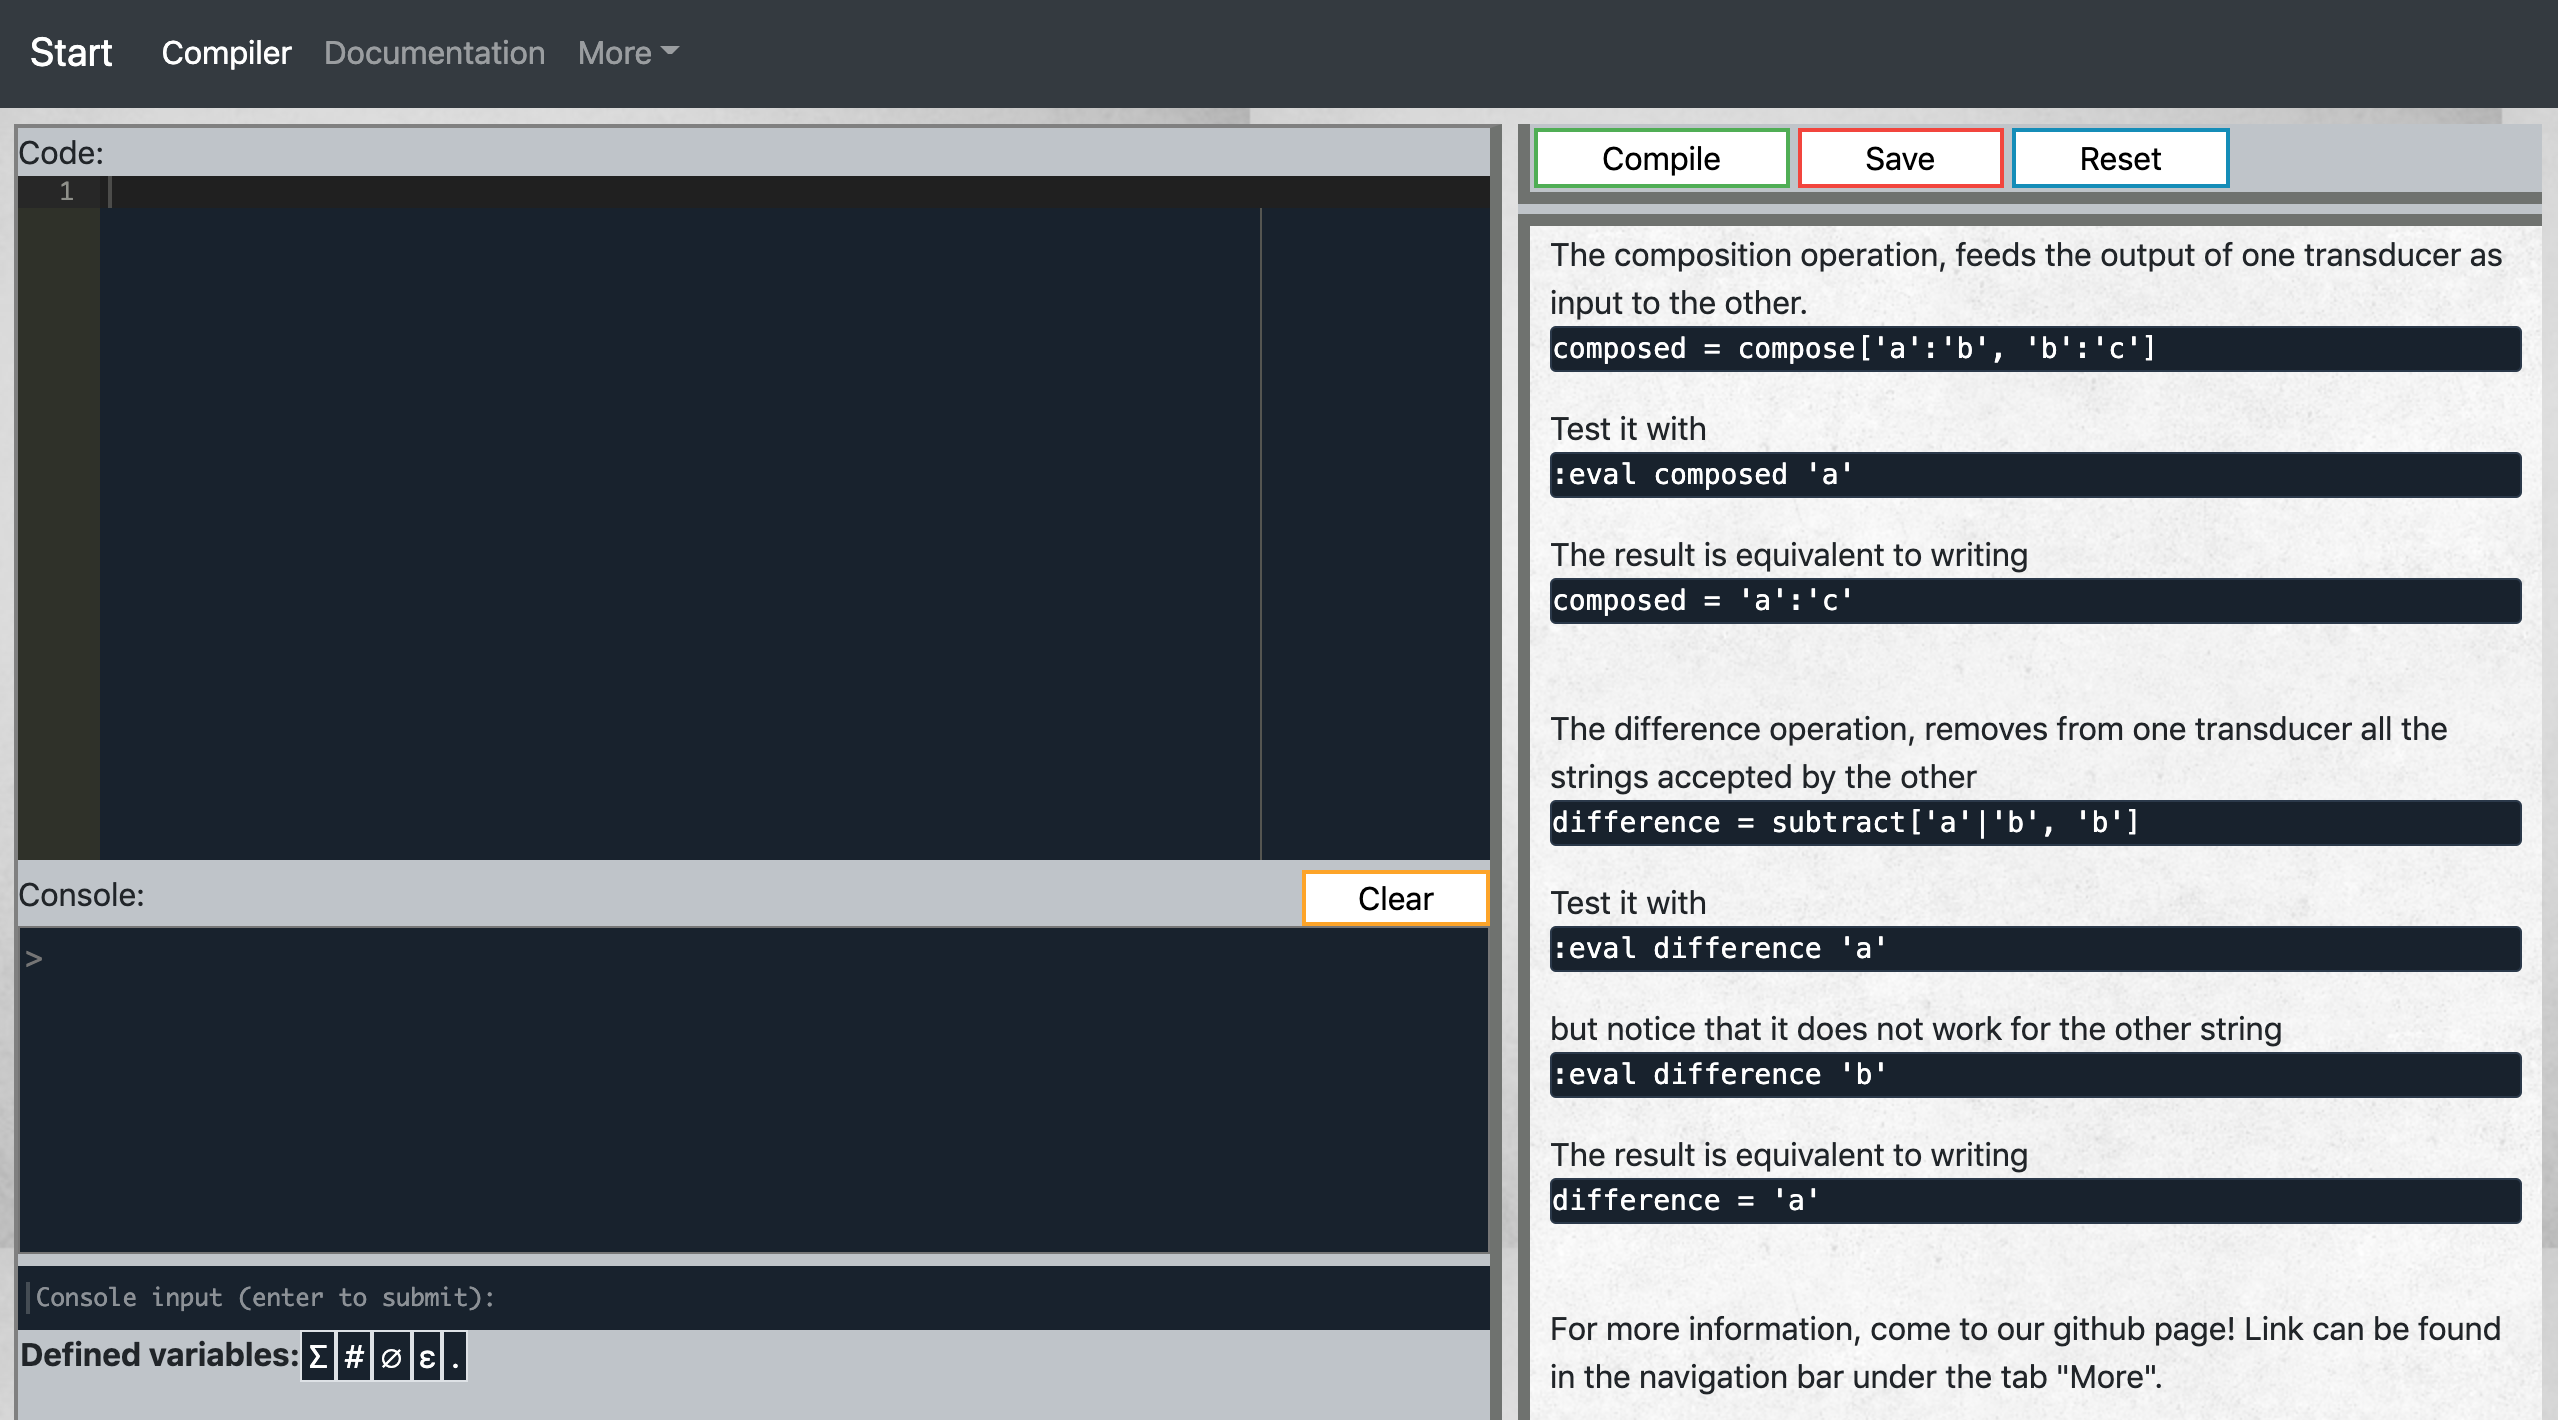
\includegraphics[scale=0.3]{web8.png}
	\caption{The final version of Solomonoff online playground. The layout inspired by several other websites and tools such as Emacs mode for Haskell, Alt-Ergo online demo and other editors}
	\label{final}
\end{figure}
Before reaching such a state we have experimented with another approach that seemed more natural for regular expressions. Figure \ref{regex} shows an example of a similar website that evaluates UNIX regexes.
\begin{figure}
	\centering
	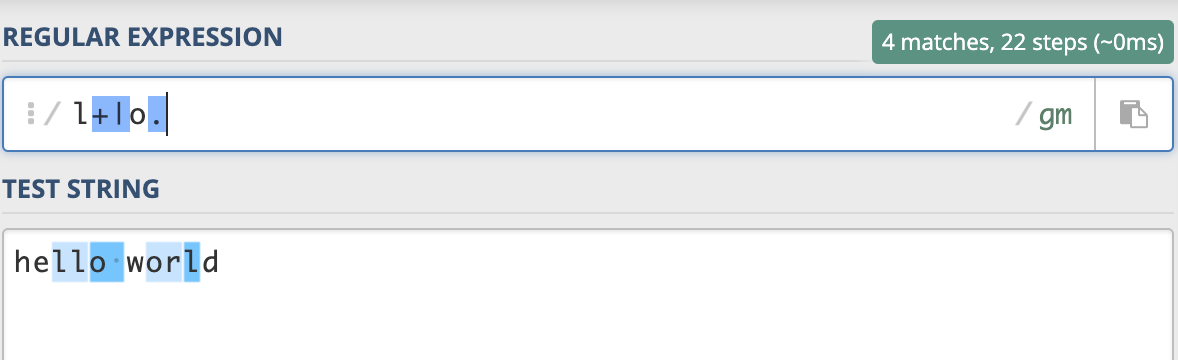
\includegraphics[scale=0.65]{regex.png}
	\caption{On this website a user can closely examine, which parts of regex correspond to a particular substring in the input.}
	\label{regex}
\end{figure}
Initially we tried to mimic such an approach with some modifications. Solomonoff is much more complex than UNIX regexes. It allows variables, functions, comments and the overall code could consist of multiple lines. Hence a dedicated multiline editor window was required like in case of Java or Haskell. Figure \ref{stage3} shows how our website looked at this stage.
\begin{figure}
	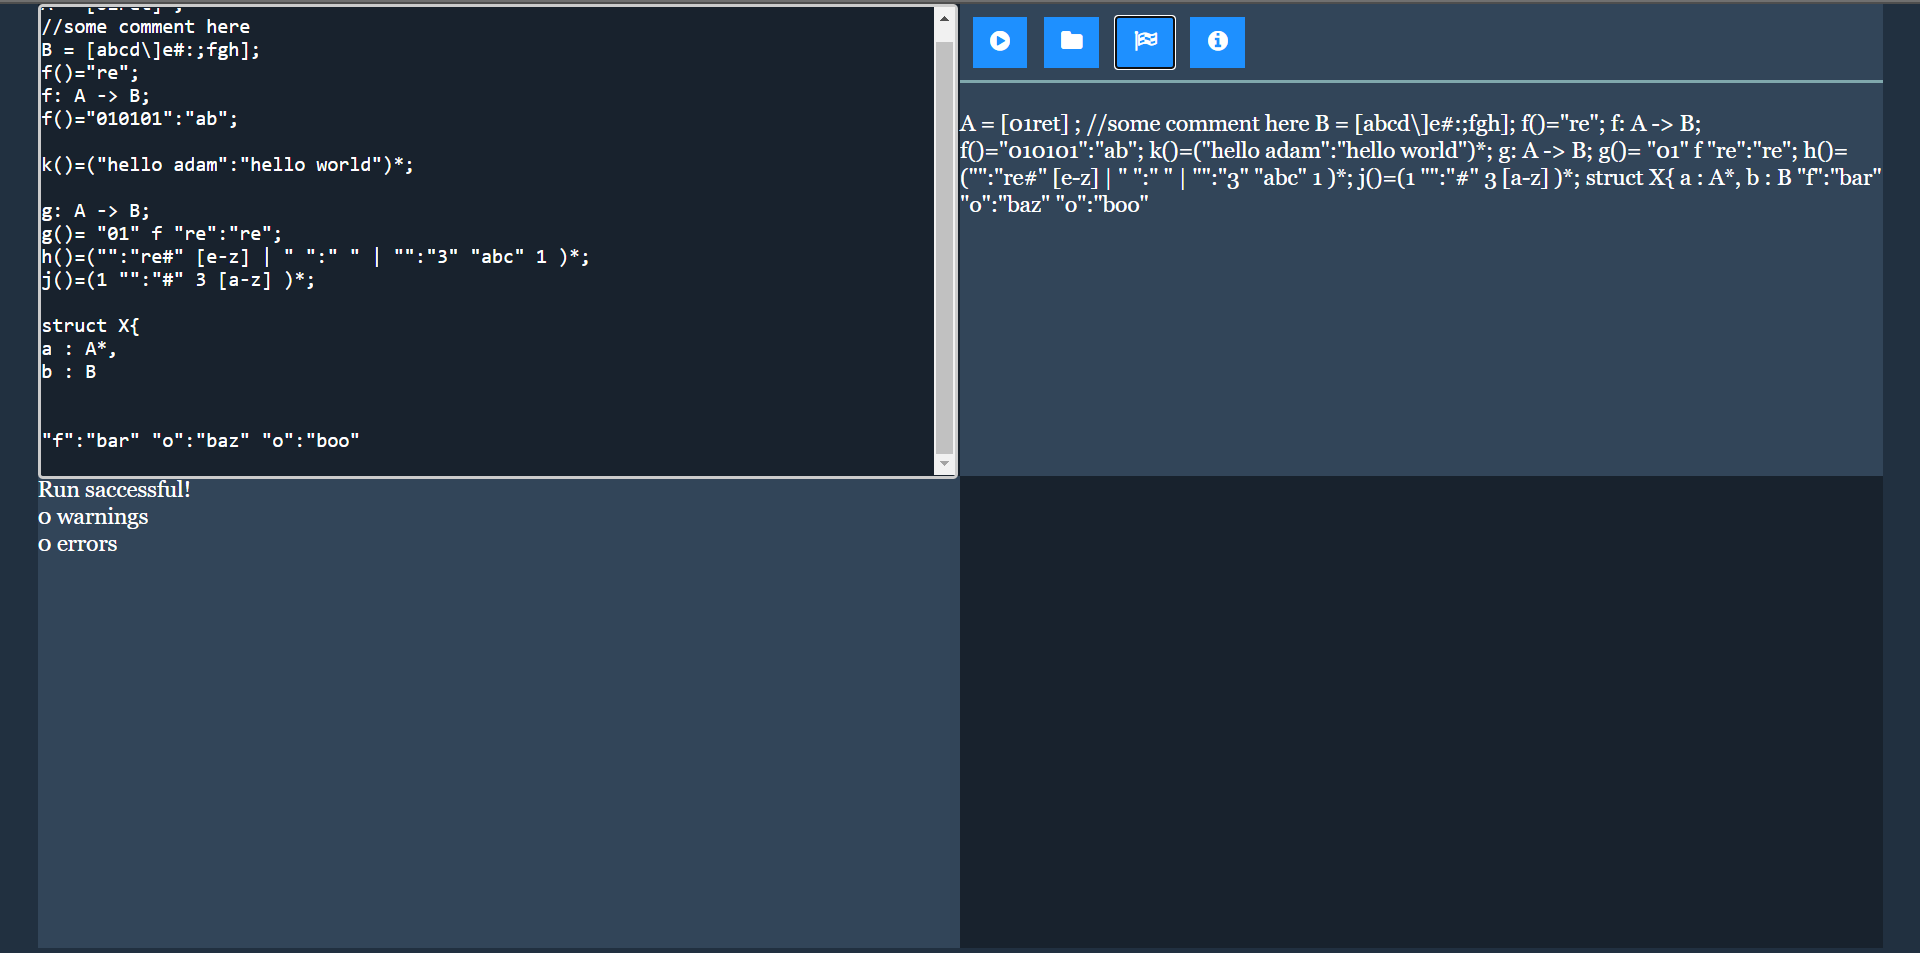
\includegraphics[scale=0.2]{web3.png}
	\caption{This early version of our website was primarily inspired by simple tools for regex investigation and debugging.}
	\label{stage3}
\end{figure}
The upper left window was dedicated to code. The lower left was meant to hold the test input string and the upper right would show the resulting transducer output. Such an approach seemed perfect at the beginning, when Solomonoff was still in early development. Over time, the language became increasingly complex. Several features were added that allowed for visualizing graphs of automata, sampling their languages, testing their formal properties and querying more complex information about them. The interface couldn't keep up with the full range of possibilities offered by the compiler. Hence, we decided to scrap the idea with two input-output windows and tried to emulate console-like REPL instead. 
It was at this point when we first tried to add a window for documentation like in figure \ref{final}. A great source of inspiration was the Alt-Ergo online demo presented in figure \ref{altergo}. It comes with many helpful examples, which can be automatically copied to the editor upon clicking on them.
\begin{figure}
	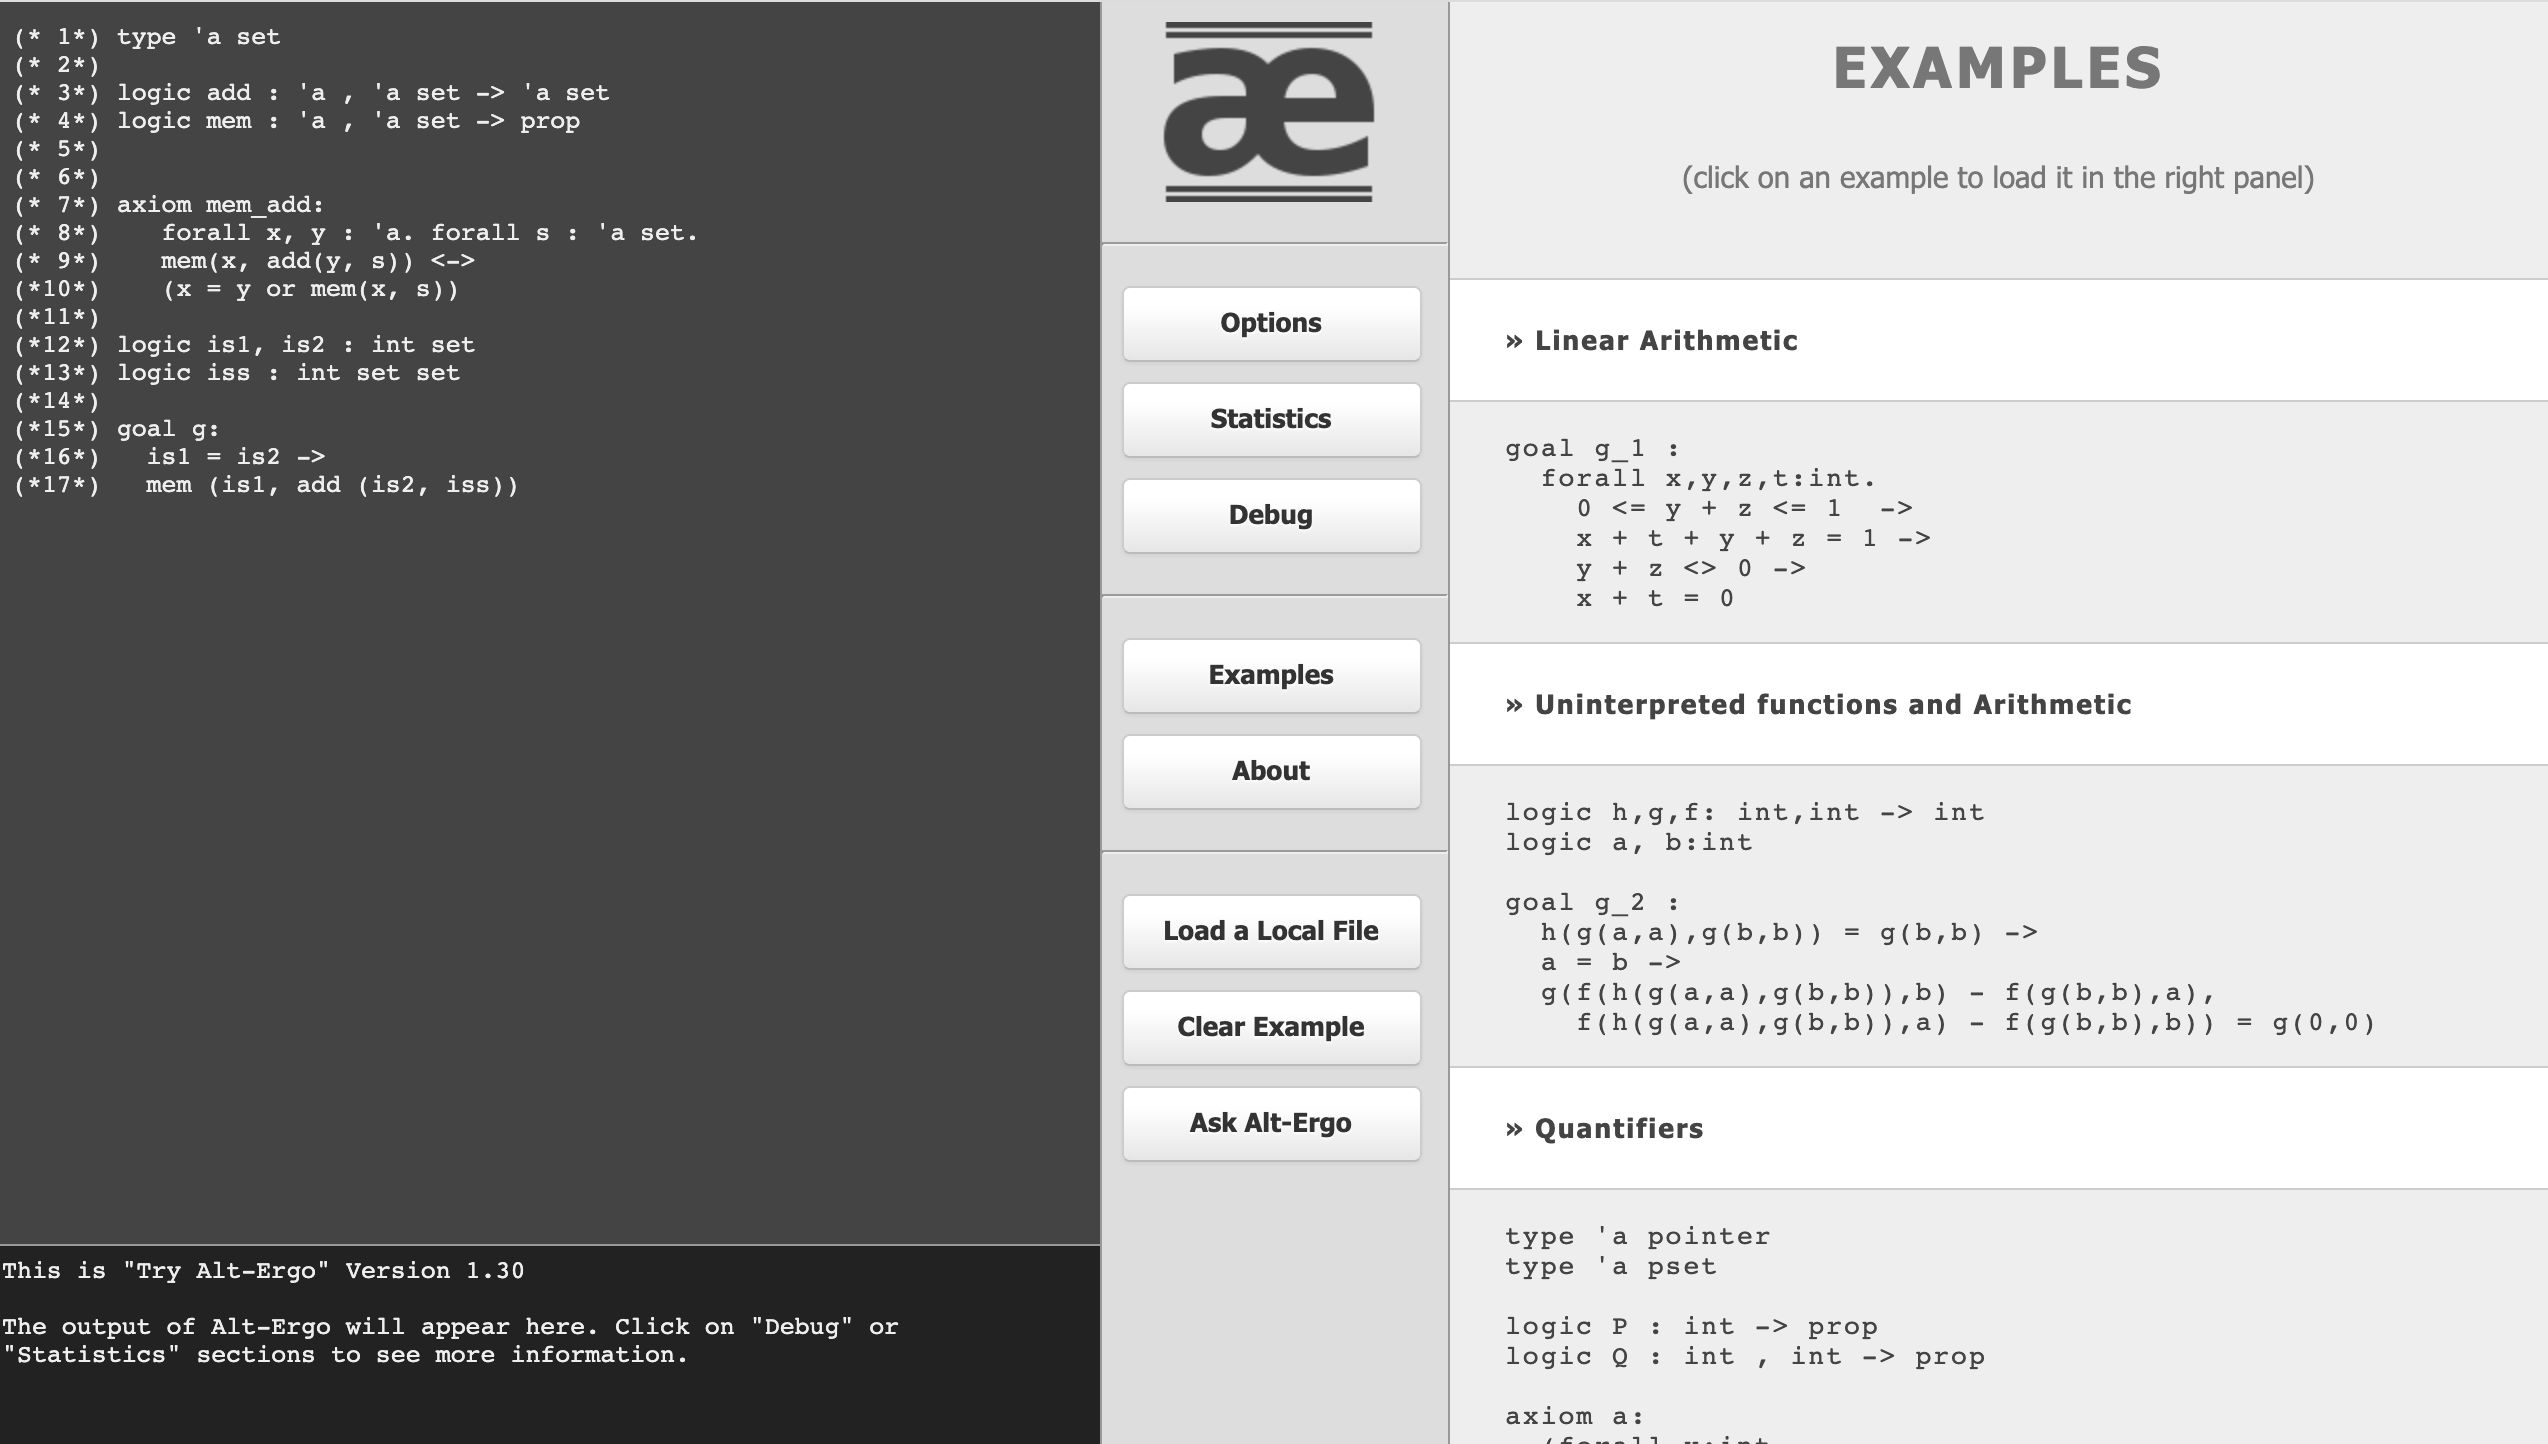
\includegraphics[scale=0.3]{alt-ergo.png}
	\caption{The Alt-Ergo is an SMT solver, which is unrelated to regular expressions but it has one thing in common with Solomonoff. They both are niche and complex tools that have a steep learning curve unaccessible to mass audiences. Alt-Ergo solved this issue by providing an online demo with interactive examples. We strived to replicate such an approach in Solomonoff.}
	\label{altergo}
\end{figure}
Later we extended this idea to a full interactive tutorial with explanations, rather than a simple list of copyable examples. 

\section{Ace editor}

At the same time as the layout of the page evolved, we also actively developed the editor itself. While initially we used a simple HTML textarea element, we soon replaced it with the Ace editor. It allowed for integrating many additional features such as syntax highlighting, auto-suggestions, code snippets and marking errors. The core component of working with Ace was the necessity of developing our own syntax highlighting. All the previously mentioned come out-of-the box for existing languages, like JavaScript, C and Python. The matters get much more complicated, when one attempts to define their custom language. Ace documentation for syntax developers tends to be rather sparse. 

There exists a common framework followed by most syntax highlighters. Their configuration consists of two main components - the highlighting rules and the styling rules. The former consist of a set of regular expressions. Any region matched by a certain expression is marked with a list of styles. Then each style decides about the colour. Many existing text editors come with their own syntax highlighter and the required configurations may differ, albeit each format could be automatically converted into any other. 

By using the Iro editor, the programmer may develop only a single set of rules and then have them automatically converted to any other syntax highlighter. This includes support for Ace, SublimeText, TextMate and Atom. Most of the other editors, like Intellij, Eclipse, Notepad++ etc. use one of the above standards. 

The general format of Iro is as follows
\begin{lstlisting}
	
	styles [] {
		
		.comment : style {
			color                 = #688557
			italic                = true
			ace_scope             = comment
			textmate_scope        = comment
			pygments_scope        = Comment
		}
		
	}
	
	main : context {
		
		: pattern {
			regex          \= (//.*)
			styles []       = .comment;
		}
		
	}
\end{lstlisting}
each pattern matches some fragment of code and assigns a style to it. Then the style defines colour and scope. The scope is later used as a hint for various other tools that rely on syntax recognition. The colours themselves are also a mere hint. The end user might use an editor that supports various colour palettes. In particular many editors come with an optional dark and light theme. Depending on the user's choice, our colouring might be overridden. Hence the assigned scope is more important than the colour hint.

Most of the language grammars are context-free and cannot be recognized with a simple regular expression. Hence syntax highlighters allow for using stacks. A good example of this are the block comments. The regular expressions that apply outside of comments should not apply inside them. Iro allows the developer to manipulate the stack using the push and pop command.
\begin{lstlisting}
	: inline_push {
		regex          \= (/\*)
		styles []       = .comment;
		default_style   = .comment
		: pop {
			regex       \= (\*/)
			styles []    = .comment;
		}
	}
\end{lstlisting}
Solomonoff's syntax highlighter uses stack to correctly recognize comments and string literals enclosed in quotes and angle brackets. The rest of the syntax highlighter is fairly simple and only matches key characters, such as equal signs, brackets, Kleene stars and union vertical pipes as well as variable identifiers.

After the syntax highlighter was developed, Iro automatically generated necessary Ace files. All those configurations are written JavaScript. In order to make them work, it's necessary to clone Ace's repository and compile the custom syntax along with the rest of sources. The compiled project needs to be hosted on the website along with remaining JavaScript files. The Ace editor can be initialized using the following lines
\begin{lstlisting}
	var editor = ace.edit("editor");
	editor.session.setMode("ace/mode/mealy");
\end{lstlisting}
where     exttt{mealy} is the name of our custom syntax.
The editor has been styled using monokai theme
\begin{lstlisting}
	editor.setTheme("ace/theme/monokai");
\end{lstlisting}
because its dark palette of colours gives the website a sharp and modern look. The dark theme is preferred by most users and is very popular nowadays. Moreover it's more relaxing to look at and doesn't irritate the eye \cite{syntax_highlighter}. This point is especially important, because Solomonoff is targeted at tech-oriented audiences, so there is a good chance that our users will spend many hours looking at the editor. 

Solomonoff comes with several built-in functions. To make the interface more intuitive and ergonomic the editor needs to provide auto-suggestions with the full range available functions. Below is a list presenting some of the more important options.
\begin{lstlisting}
	editor.setOptions({
		enableBasicAutocompletion: [{
			getCompletions: (editor, session, pos,
			prefix, callback) => {
				callback(null, [{
					name: 'subtract[',
					value: 'subtract[]',
					score: 1,
					meta: 'difference of two languages'
				},
				{
					name: 'rpni!(',
					value: 'rpni!()',
					score: 1,
					meta: 'RPNI inference algorithm'
				},
				{
					name: 'rpni_mealy!(',
					value: 'rpni_mealy!()',
					score: 1,
					meta: 'RPNI for Mealy machines'
				},
				{
					name: 'ostia!(',
					value: 'ostia!()',
					score: 1,
					meta: 'OSTIA inference for transducers'
				},
				{
					name: 'compose[',
					value: 'compose[]',
					score: 1,
					meta: 'transducer composition'
				},
				{
					name: 'inverse[',
					value: 'inverse[]',
					score: 1,
					meta: 'transducer inversion'
				}
				]);
			},
		}],
		enableSnippets: true,
		enableLiveAutocompletion: true
	});
\end{lstlisting}
The     exttt{value} field is the text that autocompletion will produce when selected. The     exttt{meta} argument provides a short explanation that will be shown to the user. We decided to set     exttt{enableLiveAutocompletion} so that the dropdown box with all available functions will automatically show up as soon as the user starts typing. Some less experienced users might not be aware that the suggestions can be triggered manually by pressing     exttt{CTRL+SPACE}. The downside is that in some contexts the autosuggestion will pop up  despite not being necessary. This could irritate some users. Perhaps the best approach would be to make the auto-suggestions configurable. A user could set the editor properties according to their own liking. The only problem was that adding user customizations would increase the complexity of the final product. Our goal was not to create a fully functioning IDE. The website is meant to work only as a showcase. Hence the final decision was to make the website as friendly to the newcomers as possible even at the cost of making the experienced users less comfortable. The general consensus was that users that like our product will quickly download the compiler locally and use it in conjunction with their own editor of choice. 

Initially, the Ace  was only used in the main editor window. The REPL console would be made of two text areas, one serving as an editable input line and the other for console output, which was permanently set as non-editable. By design, the REPL commands could only be used in console and placing them in the main editor would only result in syntax errors. For instance
\begin{lstlisting}
	:eval f 'input'
\end{lstlisting}
would only work in REPL, despite not being a valid Solomonoff code per se. As auto-suggestions were added, it became apparent that showing  REPL commands tin main editor would be very misleading
\begin{lstlisting}
	editor.setOptions({
		enableBasicAutocompletion: [{
			getCompletions: (editor, session, pos,
			prefix, callback) => {
				callback(null, [
				... 
				{
					name: ':eval',
					value: ':eval',
					score: 1,
					meta: 'evaluate transducer'
				}
				...
				]);
			},
		}],
		enableSnippets: true,
		enableLiveAutocompletion: true
	});
\end{lstlisting}
On the other hand, not showing any hints related to REPL commands would seem like a major shortcoming of the online playground. To address this issue it was later decided tha the REPL input line should also use Ace. As a result the website ended up with two instances of Ace editor. Both are very similar to each other. The only difference being that auto-suggestions in REPL input would also display REPL commands, whereas the main code editor would not.

Using Ace in REPL input also happened to solve another problem. Every REPL command would have their own format of argument. For example the     exttt{:eval} would take the transducer name and then some input string. The visualization only needs transducer name
\begin{lstlisting}
	:vis f
\end{lstlisting}
The most unintuitive is the random sample command which has two possible formats
\begin{lstlisting}
	:rand_sample f of_size 10
\end{lstlisting}
and
\begin{lstlisting}
	:rand_sample f of_length 10
\end{lstlisting}
The former generates 10 random member strings, whereas the latter generates all member strings up to length of 10.
The     exttt{of\_size} and     exttt{of\_length} argument decides which of the two modes of generation to use. The initial idea to address this issue was to add user help displayed by the     exttt{:?} command.
\begin{lstlisting}
	> :?
	:vis [ID]
	Shows graph diagram of automaton
	:rand_sample [ID] [of_size/of_length] [NUM]
	Generates random sample of input:output pairs produced 
	by ths transducer
	:ls
	Lists all currently defined transducers
	:clear
	Clears REPL console
	:run [ID] [STRING]
	Runs pipeline for the given input
	:unset [ID]
	Deletes a variable
	:is_det [ID]
	Tests whether transducer is deterministic
	:eval [ID] [STRING]
	Evaluates transducer on requested input
	...
\end{lstlisting}
The user could then consult this cheat sheet to determine the format of arguments for each command. Such a solution was simple but it certainly didn't make for the most ergonomic user interface. With Ace it became possible to use code snippets instead.
Below are a few examples.
\begin{lstlisting}
	getCompletions: (editor, session, pos, prefix, callback) => {
		callback(null, [
		{
			name: ':eval',
			value: ':eval',
			snippet: ':eval ${1:transducer_name} \'${2:input_string}\'',
			score: 1,
			meta: 'evaluate transducer'
		},
		{
			name: ':rand_sample of_size',
			value: ':rand_sample',
			snippet: ':rand_sample ${1:transducer_name} of_size ${2:number}',
			score: 1,
			meta: 'randomly generate sample'
		},
		{
			name: ':rand_sample of_length',
			value: ':rand_sample',
			snippet: ':rand_sample ${1:transducer_name} of_length ${2:number}',
			score: 1,
			meta: 'randomly generate sample'
		},
		]);
	}
\end{lstlisting}
The structure of arguments for each command was intuitively encoded in form
of blanks that need to be filled in each snippet. Each blank is specified using the \texttt{\$\{\}} braces.

\section{WebAssembly}

WebAssembly \cite{webassembly} is a technology 
that provides a new type of code 
that can be run in modern web browsers, 
providing new functionality and significant 
performance improvements. The code 
for WebAssembly is not meant to be 
written by hand, rather it is designed 
to compile efficiently from low-level 
source languages
such as C, C++, 
Rust, and so on.

WebAssembly allows code
written
in 
different languages
to run in web applications 
at near natural speed \cite{webassembly_speed,webassembly_speed2,webassembly_speed3}. 
This is of great importance 
for the web platform, as 
it previously could not be done.

Moreover, it's not necessary to know how to create WebAssembly code in order to use it. WebAssembly modules can be imported into a web application (or Node.js), and functions can be exported from them for use via JavaScript. JavaScript frameworks can use WebAssembly modules to gain tremendous performance benefits and new features, while making their functionality readily available to web developers.


The early versions of Solomonoff compiler were written in C. With help of Emscripten it was possible to then port the code to WebAssembly and call every function directly from JavaScript. Such a solution was preferable, because everything worked on client-side and we could host the website free-of-charge on GitHub
Pages. The WASM interface exposed two functions
\begin{lstlisting}
	function compile(){
		console.log(input.value)
		Module.ccall('compile',
		'void',
		['string'], 
		[input.value])
	}
	function runMealy(){
		console.log(output.value)
		var c = Module.ccall('run_global',
		'string',
		['string'], 
		[output.value])
		console.log(c);
		output.value = c;
	}
\end{lstlisting}
First one received a string of source code and the other executed defined transducer. 
Emscripten also generated a layer of JavaScript code in
\begin{lstlisting}
	<script async type="text/javascript" src="web_mealy_compiler.js"></script>
\end{lstlisting}
that smoothened the process of WebAssembly integration.
At that stage, the compiler was simple and such a minimalist API was enough. Later a lot of new functionalities were added and the project requirements shifted to Java. Several approaches for compiling Java code to WASM were attempted but with unsatisfying results.

The first framework we attempted to use was JWebAssembly. We successfully compiled and integrated toy projects but as complexity increased, the limitations became more apparent. The project page itself admitted that JWebAssembly is not yet production ready. Parts of Java standard library were missing, exceptions and threads had limited support and any attempts at converting our compiler to WASM resulted in uncountable of errors.

The next library we attempted was CheerpJ. It was the most promising option. The project compiled successfully and could run in the browser. The problem was that support for WASM is still at an experimental stage and instead CheerpJ generated JavaScript transcription of our code wrapped in heavyweight runtime. The framework is a commercial product and is primarily targeted at porting Swing/JavaFX applications to the browser. There was no documentation explaining how to expose JavaScript API or how to call any Java functions programmatically. There was also no way of manually writing HTML and CSS. Instead the produced applications mimicked typical desktop graphical interface. If we chose to use CheerpJ, we'd be forced to write a user interface in Java Swing technology.

The last available option was to use TeaVM\  \cite{teavm}. It suffered similar problems to JWebAssembly. Parts of the Java standard library were not supported. Parts of compiler code had to be rewritten to use workaround functions. For instance
the
\begin{lstlisting}
	X x = hashMap.computeIfAbsent(k,key->new X());
\end{lstlisting}
had to be rewritten as
\begin{lstlisting}
	if(hashMap.conatinsKey(k)){
		x = hashMap.get(k);
	}else{
		x = new X();
		hashMap.put(k,x);
	}
\end{lstlisting}
Another problem was with porting all the libraries and dependencies.
Parts of ANTLR\  \cite{antlr} code could not be compiled and we resorted to cloning the original ANTLR repo and manually rewriting parts of its code. Clever workarounds had to be implemented but in some cases, the code could not work in the browser in any form and had to be removed.
After enough modifications, our code compiled successfully.
When ran in the browser, the execution time was prohibitively slow and even the simplest tasks could not be completed in a satisfying time.

As a result, we were forced to forego the idea of compiling Java to WASM and switched to using backend instead. Java has a long and extensive history of being used as a server-side language with a plethora of tools and frameworks available - Spring being one of the most popular.


